\documentclass{jarticle}
 
\usepackage[dvipdfmx]{graphicx}
\usepackage{tikz}
 
\usepackage{amsmath}	% required for `\align*' (yatex added)
\begin{document}


\section{関数のグラフ}
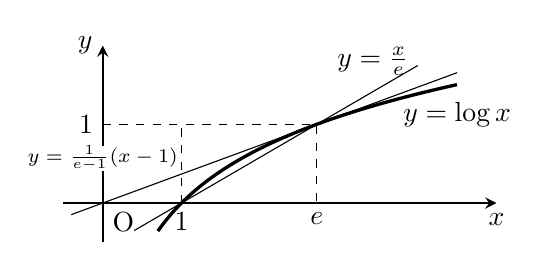
\begin{tikzpicture} 
   % 座標軸
   \draw [thick, -stealth](-0.5,0)--(5,0) node [anchor=north]{$x$};
   \draw [thick, -stealth](0,-0.5)--(0,2) node [anchor=east]{$y$};
   \node [anchor=north west] at (0,0) {O};
 
   % y=log(x)
   \draw [very thick, domain=0.7:4.5, samples=200] plot(\x, {ln(\x)});
   \node [anchor=north] at (4.5,1.4){$y=\log x$};
 
   % y=x/e
   \draw [domain=-0.4:4.5] plot(\x,\x/e);
   \node [anchor=east] at(4,1.8){$y=\frac{x}{e}$};
 
   % y=(x-1)/(e-1)
   \draw [domain=0.4:4] plot(\x, {(\x-1)/(e-1)});
   \node [anchor=south, font=\scriptsize, fill=white, inner sep=0pt] at(0,0.4){$y=\frac{1}{e-1}(x-1)$};
 
   % 補助線
   \draw [dashed](0,1) node [anchor=east]{$1$}--(e,1)--(e,0) node[anchor=north]{$e$};
   \draw [dashed](1,0) node [anchor=north]{$1$}--(1,1);
\end{tikzpicture}

\begin{tikzpicture}
  %点の設定
  \coordinate (A) at (1,1);
  \coordinate (B) at (2,1);
  \coordinate (C) at (2,2);
  \coordinate (D) at (1,3);
  \draw (A) --(B) --(C) --(D);
\end{tikzpicture}


  %塗りつぶし
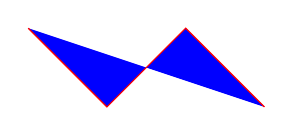
\begin{tikzpicture}
 \filldraw [draw=red,fill=blue](0,1) -- (1,0) -- (2,1) --(3,0);
\end{tikzpicture}

 %閉じた線分にはcycleをつける
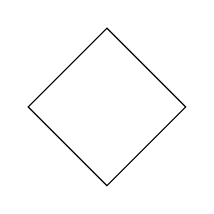
\begin{tikzpicture}
 \draw (0,1)--(1,0)--(2,1)--(1,2)--cycle;
\end{tikzpicture}


  %長方形
 \begin{tikzpicture}
   \draw (0,0) rectangle (2,2);
  \end{tikzpicture}

 %グリッド
 %help linesオプションで線の色と太さが補助専用になる.
 %stepオプションでグリッド感覚の調整が可能
 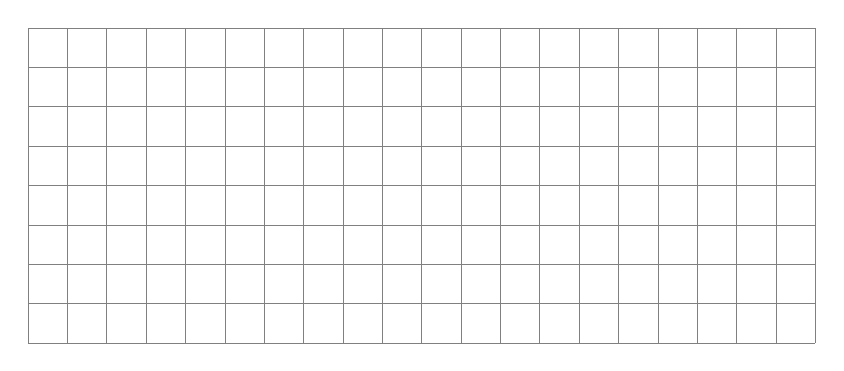
\begin{tikzpicture}
   \draw[help lines, step=0.5] (0,0) grid (10,4);
  \end{tikzpicture}


\section{ベジェ曲線}
 %ベジェ曲線の使い方
ベジェ曲線は,端点P1$(x_1,y_1)$,P2$(x_4,y_4)$,および制御点C1$(x_2,y_2)$,C2$(x_3,y_3)$に対して
\begin{align*}
 x&=(1-t)^3x_1+3(1_t)^2tx_2+3(1-t)t^2x_3+t^3x_4 \\
 y&=(1-t)^3y_1+3(1_t)^2ty_2+3(1-t)t^2y_3+t^3y_4 \\
\end{align*}
で定義される曲線である.

  %scope環境はtikzpicture環境の中にlocalな環境を作ることができる.
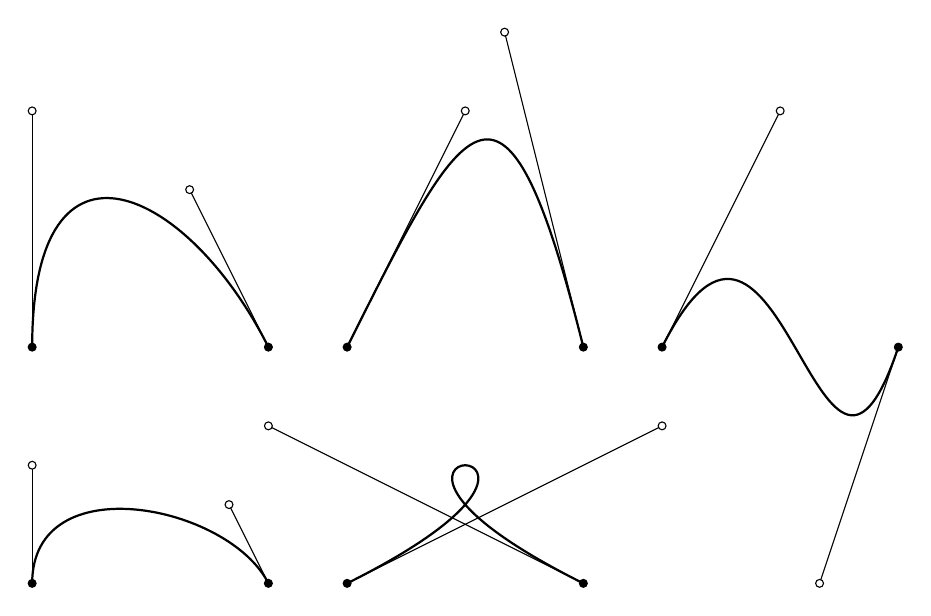
\begin{tikzpicture}
\begin{scope}
 %座標の設定
\coordinate (P1) at (0,0); %≪座標1≫
\coordinate (C1) at (0,3); %≪制御点1≫
\coordinate (C2) at (2,2); %≪制御点2≫
\coordinate (P2) at (3,0); %≪座標2≫
 %各種曲線
\draw[thick] (P1) .. controls (C1) and (C2) .. (P2); %ベジェ曲線
\draw (P1)--(C1); %補助線
\draw (C2)--(P2); %補助線
 %点の強調
\filldraw (P1) circle[radius=0.5mm];
\filldraw[fill=white] (C1) circle[radius=0.5mm];
\filldraw[fill=white](C2) circle[radius=0.5mm];
\filldraw (P2) circle[radius=0.5mm];
\end{scope}

\begin{scope}[xshift=4cm] %xshiftオプションはscope内の図形をtikzpicture環境内で右向きに平行移動
\coordinate (P1) at (0,0);
\coordinate (C1) at (1.5,3);
\coordinate (C2) at (2,4);
\coordinate (P2) at (3,0);

\draw[thick] (P1) .. controls (C1) and (C2) .. (P2); %ベジェ曲線
\draw (P1)--(C1);
\draw (C2)--(P2);

\filldraw (P1) circle[radius=0.5mm];
\filldraw[fill=white] (C1) circle[radius=0.5mm];
\filldraw[fill=white] (C2) circle[radius=0.5mm];
\filldraw (P2) circle[radius=0.5mm];
\end{scope}

\begin{scope}[xshift=8cm] %xshiftオプションはscope内の図形を右向きに平行移動
\coordinate (P1) at (0,0);
\coordinate (C1) at (1.5,3);
\coordinate (C2) at (2,-3);
\coordinate (P2) at (3,0);

\draw[thick] (P1) .. controls (C1) and (C2) .. (P2); %ベジェ曲線
\draw (P1)--(C1);
\draw (C2)--(P2);

\filldraw (P1) circle[radius=0.5mm];
\filldraw[fill=white] (C1) circle[radius=0.5mm];
\filldraw[fill=white] (C2) circle[radius=0.5mm];
\filldraw (P2) circle[radius=0.5mm];
\end{scope}

\begin{scope}[yshift=-3cm] %xshiftオプションはscope内の図形を上向きに平行移動
\coordinate (P1) at (0,0);
\coordinate (C1) at (0,1.5);
\coordinate (C2) at (2.5,1);
\coordinate (P2) at (3,0);
\draw[thick] (P1) .. controls (C1) and (C2) .. (P2); %ベジェ曲線
\draw (P1)--(C1);
\draw (C2)--(P2);
\filldraw (P1) circle[radius=0.5mm];
\filldraw[fill=white] (C1) circle[radius=0.5mm];
\filldraw[fill=white] (C2) circle[radius=0.5mm];
\filldraw (P2) circle[radius=0.5mm];
\end{scope}

\begin{scope}[xshift=4cm, yshift=-3cm]
\coordinate (P1) at (0,0);
\coordinate (C1) at (4,2);
\coordinate (C2) at (-1,2);
\coordinate (P2) at (3,0);
\draw[thick] (P1) .. controls (C1) and (C2) .. (P2); %ベジェ曲線
\draw (P1)--(C1);
\draw (C2)--(P2);
\filldraw (P1) circle[radius=0.5mm];
\filldraw[fill=white] (C1) circle[radius=0.5mm];
\filldraw[fill=white] (C2) circle[radius=0.5mm];
\filldraw (P2) circle[radius=0.5mm];
\end{scope}
\end{tikzpicture}

%ベジェ曲線でも相対座標が使える.
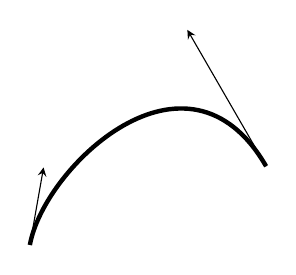
\begin{tikzpicture}
 \coordinate (P1) at (0,0);
 \coordinate (P2) at (3,1);
 \draw[ultra thick] (P1).. controls +(80:1cm) and +(120:2cm) ..(P2);
 \draw[-stealth] (P1) -- +(80:1cm);
 \draw[-stealth] (P2) -- +(120:2cm);
\end{tikzpicture}

%ハート形
\begin{tikzpicture}
 %座標
 \coordinate (P1) at (3,0);
 \coordinate (P2) at (0,0);
 \coordinate (P3) at (-3,0);
 \coordinate (P4) at (0,-4);
  
 %ハート
 \filldraw[ultra thick, fill=pink] (P1) node [anchor=west] {P1}
  .. controls +(80:2.5cm) and +(90:2.5cm) .. (P2) node [anchor=north]{P2}
  .. controls +(90:2.5cm) and +(100:2.5cm) .. (P3) node [anchor=east]{P3}
  .. controls +(280:2.5cm) and +(110:0.5cm) .. (P4) node [anchor=north]{P4}
  .. controls +(70:0.5cm) and +(260:2.5cm) .. (P1);
\end{tikzpicture}



\section{円,楕円の書き方}
%円弧,楕円弧
円弧の表し方は
	
(≪座標P≫) arc[start angle=≪開始角α≫, end angle=≪終了角β≫, radius=≪半径r≫]

または
(≪座標P≫) arc (≪開始角α≫:≪終了角β≫:≪半径r≫)

である.座標Pが開始角$\alpha$に対応する.

\begin{tikzpicture}
 \draw (0,0) -- (6,0) arc (120:270:2cm) -- ++(-4,0);
\end{tikzpicture}

同様に,円は 
(≪座標1≫) circle[radius=≪半径r≫]
(≪座標1≫) circle(≪半径r≫)
で,座標1を中心とする半径rの円を表す.



\section{放物線}
%放物線

 (≪座標1≫) parabola (≪座標2≫)
で座標1を頂点として,座標2を通る放物線を表す.

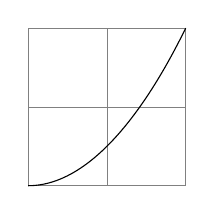
\begin{tikzpicture}
 \draw[help lines] (0,0) grid (2,2);
 \draw (0,0) parabola(2,2);
\end{tikzpicture}


これでは頂点からしか書けないが,より一般的に指定するには
(≪座標1≫) parabola bend(≪座標2=頂点≫) (≪座標3≫)
とすれば良い.ただしこれは二つの放物線を合わせたものであることに注意すること.




\end{document}
